\newif\ifColor
% Add \Colortrue to settings.tex to use color
% Otherwise, will show a primarily grayscale version of the document for printing

\input{settings.tex}


\documentclass[11pt,oneside,a4paper]{article}
\usepackage{enumitem}

\usepackage{tikz}
\usepackage{natbib}
\usepackage{breakcites} % Do Not let citations break out of the text frame
\usepackage{microtype} % Get rid of some frame busts automatically
% Note: if microtype causes error on ubuntu, run
% sudo apt-get install cm-super
\title{Assignment 2}
\author{CMPS 392}
\date{}
% \setcounter{tocdepth}{1}

\pdfobjcompresslevel=0

\usepackage{zref-abspage}

\setcounter{secnumdepth}{3} % Number subsubsections, because we reference them,
% so the reader needs numbers to find the correct place.


\usepackage[vcentering,dvips]{geometry}
\geometry{papersize={7in,9in},bottom=3pc,top=5pc,left=5pc,right=5pc,bmargin=4.5pc,footskip=18pt,headsep=25pt}


%%% Packages %%%
\usepackage{epsfig}
\usepackage{subfigure}
\usepackage[utf8]{inputenc}

% Needed for some foreign characters
\usepackage[T1]{fontenc}

\usepackage{amsmath}
\usepackage{subfigure}
\usepackage{amsfonts}
\usepackage{amsthm}
\usepackage{multirow}
\usepackage{colortbl}
\usepackage{booktabs}
% This allows us to cite chapters by name, which was useful for making the
% acknowledgements page
\usepackage{nameref}
% Make sure there is a space between the subsection number and subsection title
% in the table of contents.
% If we do not do this we end up with 2 digit subsection numbers colliding with
% the title.
% See https://tex.stackexchange.com/questions/7853/toc-text-numbers-alignment/7856#7856?newreg=d2632892dd0345f388619f12fa794b11
% \usepackage[tocindentauto]{tocstyle}
% \usetocstyle{standard}

\usepackage{bm}


\usepackage{float}
\newcommand{\boldindex}[1]{\textbf{\hyperpage{#1}}}
\usepackage{makeidx}\makeindex
% Make bibliography and index appear in table of contents
\usepackage[nottoc]{tocbibind}
% Using the caption package allows us to support captions that contain "itemize" environments.
% The font=small option makes the text of captions smaller than the main text.
\usepackage[font=small]{caption}

% Used to change header sizes
\usepackage{fancyhdr}



% \usepackage[chapter]{algorithm}
\usepackage{algorithmic}
% Include chapter number in algorithm number
% \renewcommand{\thealgorithm}{\arabic{chapter}.\arabic{algorithm}}


\theoremstyle{definition}
\newtheorem{example}{Example}[section]

% Define the P table cell environment
% It is the same as p, but centers the text horizontally
\usepackage{array}
\newcolumntype{P}[1]{>{\centering\arraybackslash}p{#1}}

% Rebuild the book document class's headers from scratch, but with different font size
% (this is for MIT Press style)
% Source: http://texblog.org/2012/10/09/changing-the-font-size-in-fancyhdr/
\newcommand{\changefont}{% 1st arg to fontsize is font size. 2nd arg is the baseline skip. both in points.
    \fontsize{9}{11}\selectfont
}
\fancyhf{}
\fancyhead[LE,RO]{\changefont \slshape \rightmark} %section
% \fancyhead[RE,LO]{\changefont \slshape \leftmark} %chapter
\fancyfoot[C]{\changefont \thepage} %footer
\pagestyle{fancy}
\input{math_commands.tex}

\usepackage[pdffitwindow=false,
pdfview=FitH,
pdfstartview=FitH,
pagebackref=true,
breaklinks=true,
\ifColor
colorlinks,
\fi
bookmarks=false,
plainpages=false]{hyperref}

% Make \[ \] math have equation numbers
\DeclareRobustCommand{\[}{\begin{equation}}
\DeclareRobustCommand{\]}{\end{equation}}

% Allow align environments to cross page boundaries.
% If we do not do this, we get weird gaps of several inches of white space
% before or after some long align environments.
\allowdisplaybreaks

\begin{document}

\setlength{\parskip}{0.25 \baselineskip}
\newlength{\figwidth}
\setlength{\figwidth}{26pc}
% Spacing between notation sections
\newlength{\notationgap}
\setlength{\notationgap}{1pc}

% \typeout{START_CHAPTER "TOC" \theabspage}
%\frontmatter


\maketitle
%\tableofcontents
%\typeout{END_CHAPTER "TOC" \theabspage}

%  \input{notation.tex}
 %\mainmatter
%  \input{commentary.tex}

\section*{Useful Formulas} 
Given:
the sigmoid function: 
$$ \sigma(x) = \frac{1} {1 + exp(-x) } $$ 
and the softplus function 
$$ \zeta(x) = log(1+exp(x) ) $$ 
Softplus means it is a soft version of  $x^+ = max(0,x) $

Plot the curves of these functions and prove the following properties: 

     $$\sigma(x) = \frac{\exp(x)}{\exp(x)+\exp(0)}$$
     $$\frac{d}{d x} \sigma(x)=  \sigma(x) (1 -  \sigma(x) ) $$
     $$1-  \sigma(x) =  \sigma(-x)$$
     $$\log \sigma(x) = - \zeta(-x) $$
     $$\forall x \in (0,1),~ \sigma^{-1}(x) = \log(\frac{x}{1-x})$$
     $$\forall x >0,~ \zeta^{-1} (x) = \log (\exp(x)-1)$$
     $$\zeta(x) = \int_{-\infty}^x \sigma(y) d y $$
     $$\zeta(x) - \zeta(-x) = x $$


 
\section*{Expectation and Variance}
Prove that the following are valid probability mass functions and compute their expectation and variance: 

\begin{itemize}
    \item   $ \displaystyle P(x) = \begin{cases}
      \phi & \text{if $x = 1$ }\\
      1 - \phi & \text{if $x = 0$}\\
    \end{cases}  \quad  \phi \in [0,1]$
\item 
$ \displaystyle P(k) = 
{n \choose k}\phi^k (1-\phi)^{n-k} \quad \text{for} \quad  0 \leq k \leq n  \quad  \phi \in [0,1]$
\item 
$ \displaystyle
 P (k) = \phi (1-\phi)^{k-1} \quad \text{for} \quad k = 1,2, \ldots  \quad  \phi \in [0,1]
$
\item $ \displaystyle  P (k) =  e^{-\lambda} \frac{\lambda^k}{k!} \quad \text{for} \quad k = 1,2, \ldots \quad  \lambda > 0  $

\end{itemize}

Prove that the following are valid probability density functions and compute their expectation and variance: 


\begin{itemize}
    \item   $ \displaystyle p(x) = \frac{1}{b-a} \quad \forall x \in (a,b) $
\item 
$ \displaystyle p(x) = \frac{1}{\sigma \sqrt{2\pi} } e^{-\frac{(x-\mu)^2}{2\sigma^2}}$

\item $ \displaystyle p(x) = \lambda e^{-\lambda x}  \quad x\geq 0, \quad \lambda >0 $
\end{itemize}


\section*{Spam detection}
Suppose you receive an e-mail message with the subject “PRIZE AWARD”. You have been keeping statistics on your e-mail, and have found that while only 10\% of the total e-mail messages you receive are spam, 50\% of the spam messages have the subject “PRIZE AWARD” and 2\% of the non-spam messages have the subject “PRIZE AWARD”. What is the probability that the message is spam?

\section*{Birthday Paradox} 
Imagine a society where families want to have the least amount of kids as long as they have a boy. What is the boys to girls ratio in such society? 

% Examples of birth gender sequences of different families:
% \begin{itemize}
% \item F,F,F,F,M
% \item M 
% \item F,F,M
% \item F,M
% \item F,F,F,F,F,F,F,F,M
% \end{itemize} 








\section*{Programming Assignment} 

We want to draw lines in a rectangular area in 2D in the most uniform way. 

\begin{figure}[!h]
    \centering
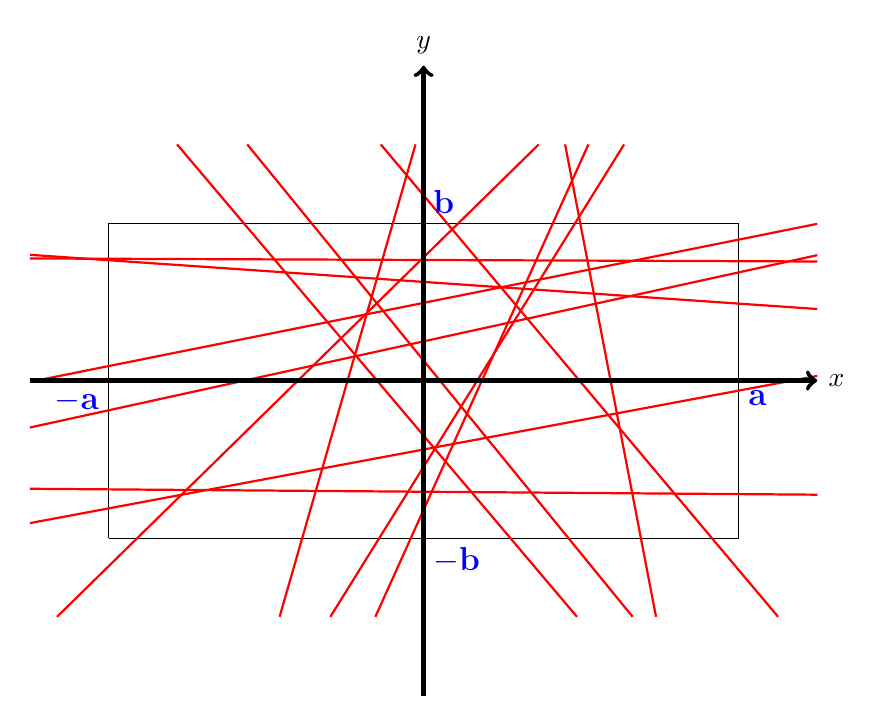
\begin{tikzpicture}
\centering
\draw (-4,-2) -- (-4,2) -- (4,2) -- (4,-2) -- (-4,-2);

-3.1313
   -0.1024
   -0.5441
    1.4631
    2.0936
    2.5469
   -2.2397
    1.7970


\draw [color=red, thick=2pt]  (1.9483,-3) --  (-3.1313,3) ;
\draw [color=red, thick=2pt]  (-1.8290,-3) -- (-0.1024,3) ;
\draw [color=red, thick=2pt]  ( 4.5022,-3) -- (-0.5441,3) ;
\draw [color=red, thick=2pt]  (-4.6555,-3) -- ( 1.4631,3) ;
\draw [color=red, thick=2pt]  (-0.6126,-3) -- ( 2.0936,3) ;
\draw [color=red, thick=2pt]  (-1.1844,-3) -- ( 2.5469,3) ;
\draw [color=red, thick=2pt]  ( 2.6552,-3) -- (-2.2397,3) ;
\draw [color=red, thick=2pt]  ( 2.9520,-3) -- (1.7970,3) ;
\draw [color=red, thick=2pt]  (-5, 1.5510) --  (5, 1.5127) ;
\draw [color=red, thick=2pt]  (-5, -1.3739) -- (5,-1.4490) ;
\draw [color=red, thick=2pt]  (-5, -1.8100) -- (5, 0.0596) ;
\draw [color=red, thick=2pt]  (-5, -0.0164) -- (5, 1.9908) ;
\draw [color=red, thick=2pt]  (-5, 1.5974) --  (5, 0.9090) ;
\draw [color=red, thick=2pt]  (-5, -0.5961) -- (5, 1.5929) ;

\draw[->,ultra thick] (-5,0)--(5,0) node[right]{$x$};
\draw[->,ultra thick] (0,-4)--(0,4) node[above]{$y$};

\node [color=blue] at (-4,0) [below left]{\large  $\mathbf{-a}$ }; 
\node [color=blue] at (4,0) [below right]{\large  $\mathbf{a}$ }; 
\node [color=blue] at (0,-2) [below right]{\large $\mathbf{-b}$ }; 
\node [color=blue] at (0,2) [above right]{\large  $\mathbf{b}$ }; 
\end{tikzpicture}
\end{figure}




Consider the following methods: 
\begin{itemize}
    \item Sample $ x_1, x_2 \sim \mathcal{U}[-a,a], \quad y_1, y_2 \sim \mathcal{U}[-b,b]$, and draw the line connecting point $(x_1, y_1)$ and $(x_2, y_2)$.
    \item Sample $r \sim \mathcal{U}[0,\sqrt{a^2+b^2}]$ and $ \theta \sim \mathcal{U}[0,2\pi]$, and draw the line at angle $\theta$ and distance $r$ from the origin. 
    \item Sample  $x \sim \mathcal{U}[-a,a], ~ y \sim \mathcal{U}[-b,b], ~ \gamma \sim \mathcal{U}[0,2\pi] $, and draw the line passing through point $(x,y)$ and having slope $\gamma$. 
\end{itemize}

Apply for $a = 2, ~b = 1$. Draw around 100 lines for each method and compare. Which one looks the most uniform to you?
If none of the above methods is satisfying, you can propose your own method.

\end{document}
